%\documentclass[10pt,handout]{beamer}
\documentclass[10pt]{beamer}
\usepackage{babel} % Anpassa efter svenska. Ger svensk logga.
\usepackage[utf8]{inputenc} % Anpassa efter linux
\usepackage{graphicx}
\usepackage{../common/beamerthemeUppsala}
%\usecolortheme{UU} % Anpassa efter UU:s frger och logga
%\hypersetup{pdfpagemode=FullScreen} % Adobe Reader ska ppna fullskrm
\setbeamertemplate{itemize items}[circle]

% \usepackage{beamerthemesplit}
\usepackage{amsmath}
\usepackage{amssymb}
% \usepackage{graphics}
% \usepackage{graphicx}
% \usepackage{epsfig}
% \usepackage[latin1]{inputenc}
 \usepackage{color}
% \usepackage{fancybox}
% \usepackage{psfrag}
% \usepackage[english]{babel}
 \setbeamertemplate{footline}{\hfill\insertframenumber/\inserttotalframenumber}

%library(tinytex)
%tlmgr_install('booktabs')
\usepackage{booktabs}

% Read in commands
% Course settings
\newcommand{\currentsemester}{Autumn 2024}

% New commands
\newcommand{\bfm}[1]   {\mbox{\boldmath{${#1}$}}}
\newcommand{\Prob}   {\mbox{\textnormal{P}}}
\newcommand{\uured}[1]{\textcolor{uured}{#1}}

% Eqds
\def\eqd{\,{\buildrel d \over =}\,}

% Math operators
\DeclareMathOperator{\E}{\mathbb{E}}
\DeclareMathOperator{\V}{\mathbb{V}}


%%%%%%%%%%%%%%%%%%%%%%%%%%%%%%%%%%%%%%%%%%%%%%%%%%%%%%%%%%%%%%%%%%

\setlength{\parskip}{3mm}
\title[]{{\color{black}Machine learning -- Block 8}}
\author[]{M{\aa}ns Magnusson\\Department of Statistics, Uppsala University}
\date{\currentsemester}


\begin{document}

\frame{\titlepage
% \thispagestyle{empty}
}

%%%%%%%%%%%%%%%%%%%%%%%%%%%%%%%%%%%%%%%%%%%%%%%%%%%%%%%%%%%%%%%%%%


\begin{frame}{This week's lectures}
\begin{itemize}
\item Introduction to Reinforcement learning
\end{itemize}
\end{frame}


%%%%%%%%%%%%%%%%%%%%%%%%%%%%%%%%%%%%%%%%%%%%%%%%%%%%%%%%%%%%%%%%%%

\section{Introduction to Reinforcement Learning}

\begin{frame}{Introduction to Reinforcement Learning}

\begin{itemize}
\item Another type of Machine Learning:
\begin{itemize}
\item Supervised Learning
\item Unsupervised Learning
\item {\color{uured} Reinforcement learning}
\end{itemize}
\pause
\item Computational approach of {\color{uured} learning from interaction}
\pause
\item Closest to human and animal learning: {\color{uured} trial, error, and planning.}
\pause
\item The learner is \emph{not} told which actions to take
\pause
\item Connections to:
\begin{itemize}
\item Game Theory
\item Control Theory
\item Multi-agent systems
\item Swarm intelligence
\item Information theory
\item Statistics
\end{itemize}
\end{itemize}

\end{frame}

\begin{frame}{Introduction to Reinforcement Learning}

\begin{itemize}
\item {\color{uured} Goal}: maximize return over a sequence of actions\pause
\item Three characteristics:
\begin{enumerate}
\item \uured{Closed-loop}: early actions affects later actions\pause
\item \uured{No instructions}\pause
\item \uured{Reward signals} over a long period of time
\end{enumerate}
\end{itemize}

\end{frame}


\begin{frame}{Recent Achievements}

\begin{figure}[h]
\centering
\only<1>{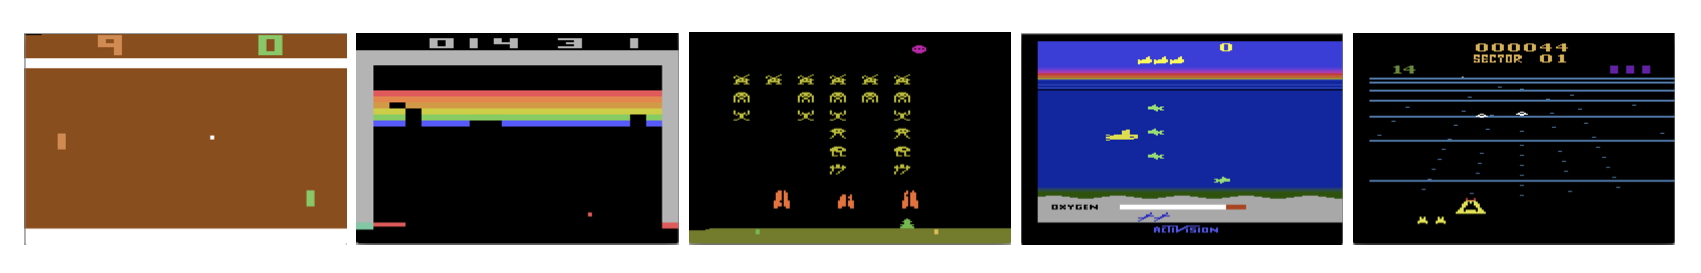
\includegraphics[width=0.99\textwidth]{fig/mnih2013rlatari}
\caption{Mnih et al (2013) "Playing Atari with Deep Reinforcement Learning"
}}
\only<2>{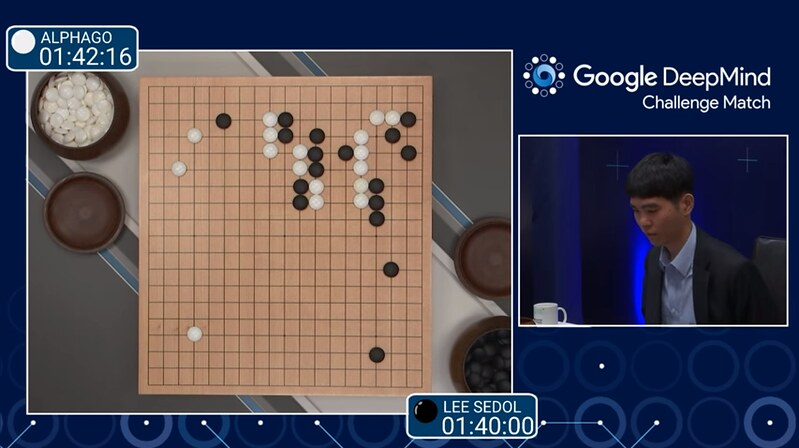
\includegraphics[width=0.99\textwidth]{fig/leesedol}
\caption{Lee Sedol vs. Alpha Go in 2016}}
\only<3>{
\includegraphics[width=0.5\textwidth]{fig/ChatGPT_logo}
\caption{ChatGPT in 2022}}
\end{figure}

\end{frame}


\begin{frame}{Recent Achievements, also }

\begin{itemize}
\item Industry automation: RL is used to reduce the energy cost of datacenter cooling\pause
\item Automated trading\pause
\item Elevator scheduling\pause
\item A/B testing and personalized recommendations
\end{itemize}

\end{frame}



\begin{frame}{The different parts in RL}

\begin{enumerate}
\item The {\color{uured} Agent}: The learning agent. \pause
\item The {\color{uured} Environment}: Where the agent performs actions.\pause
\item {\color{uured} Actions}: Made by the agent and affects the environment.\pause
\item {\color{uured} Reward}: The evaluation of an action. A scalar value. Pleasure and pain.\pause
\item {\color{uured} Return}: The aggregated reward over a long period.
\end{enumerate}

\end{frame}



\begin{frame}{The different parts in RL}

\begin{enumerate}
\item Agents:
\begin{enumerate}
\item Have a {\color{uured} goal} (maximize return)
\item {\color{uured} Sense} aspect of their environment
\item Choose {\color{uured} actions}
\item Possibility to {\color{uured} improve performance over time}
\end{enumerate}
\pause
\item Usually an {\color{uured} uncertainty} about the environment
\item Represent uncertainty of environment: {\color{uured} Probability}
\end{enumerate}

\end{frame}


\begin{frame}{Sub-elements of agents}

\begin{enumerate}
\item {\color{uured} Policy}: How the agent choose actions. Determines behaviour.
\item {\color{uured} Model}: The agent's model of the environment. Used for {\color{uured} planning}\pause
\item {\color{uured} Value function}: The long-term value (the expected long-term return following a policy)
\end{enumerate}
\pause
\begin{itemize}
\item Outside agent: {\color{uured} Reward signal}: The instant value of an action\pause
\item Problem: {\color{uured} Balance} the trade-off between long-term and short-term rewards
\end{itemize}

\end{frame}

\begin{frame}{Supervised, Unsupervised and Reinforcement Learning}

\begin{enumerate}
\item Static vs. Dynamic \pause
\item No Gold Standard \pause
\item Multiple-Decision Process: Return vs. reward\pause
\item Need for exploration\pause
\item Evaluates actions - not only instruct actions
\end{enumerate}

\end{frame}

\begin{frame}{Exploration vs Exploitation}

\begin{itemize}
\item {\color{uured} Goal}: Maximize the return (the total reward), i.e.\pause
\item {\color{uured} Exploit} the best actions\pause
\item {\color{uured} Explore} to know the best actions
\end{itemize}

\end{frame}

\begin{frame}{Evolution vs Learning}

\begin{itemize}
\item Set a policy without learning: {\color{uured} Evolutionary} Methods
\item Good when agent cannot sense the environment\pause
\item {\color{uured} Example}: Bacteria don't learn, they evolve
\end{itemize}

\end{frame}


\begin{frame}{Setting the goal for the Agent}

\begin{itemize}
\item Setting the goal: {\color{uured} defining the reward} signal (reward function)
\item {\color{uured} Example}: If you want the agent to do something quick, give -1 per action.\pause
\item We should give rewards for correct {\color{uured} behaviour}
\item Do {\color{uured} not} use reward to guide {\color{uured} how} to reach the goal
\item \href{https://openai.com/blog/faulty-reward-functions/}{{\color{blue} Be careful what you wish for...}}
\end{itemize}

\end{frame}


\section{Bandits}
\frame{\sectionpage}
% TODO: Add policy also in the bandit part ie that the choosing of A is a policy, the greedy policy, epsilon policy etc


\begin{frame}{The $k$-armed bandit problem}

\begin{itemize}
% TODO: Find an image here.
\item {\color{uured} Goal}: Maximize the total or average reward after $N$ actions\pause
\item {\color{uured} The actions}: Choose between $k$ arms, i.e. $A_t \in \{1,...,k \}$\pause
\item The reward signal:
\[
R_{t} \sim p(R_t|a)\,,
\]
where $\mathbb{E}(R_{t}|A_t = a) = q^\star(a)$.\pause
\item $q^\star(a)$ is {\color{uured} unknown}.\pause
\item The estimated (expected) value if action $a$ at step $t$: $Q_t(a)$.\pause\vspace{3mm}
\item This is a {\color{uured} tabular} method/problem: \\ We can represent the actions in a table.
\item Tabular methods works in small problems\\ e.g. A/B testing and dynamic web pages.
\end{itemize}

\end{frame}

\begin{frame}{Exploration vs. Exploitation}

\begin{itemize}
% TODO: Find an image here.
\item Two types of actions:
\begin{enumerate}
\item Exploitation: Choose the action with highest expected reward (short term)
\item Exploration: Choose action to improve $Q_t(a)$, but reduces the reward (long term)
\end{enumerate}
\item The {\color{uured} conflict} between exploration and exploitation
\end{itemize}

\end{frame}


\begin{frame}{$\epsilon$-greedy}

\begin{itemize}
\item $\epsilon$-greedy: $P(\text{exploration}) = \epsilon$ \pause
\begin{itemize}
\item Exploitation:
\[
A_t = \arg \max_a Q_t(a)
\]
\pause
\item Exploration:
\[
A_t \sim U(1,...k)
\]
\pause
\end{itemize}
\item $Q_1(a) = 0$ (or used to encourage initial exploration)\pause
\item For any $\epsilon > 0$, $Q_t(a) \rightarrow q^\star(a)$
\end{itemize}

\end{frame}

\begin{frame}{$\epsilon$-greedy}

\begin{itemize}
\item We estimate $q^\star(a)$ using $Q_t(a)$ as
\[
Q_T(a) = \frac{1}{N(a)} \sum^{T-1}_t R_{t,A_t=a}\,,
\]
where $N(a)$ is the total number of times action $a$ has been taken.
\pause
\item When should we explore?
\begin{itemize}
\item Large $V(R_t)$\pause
\item Large $\mathcal{A}$\pause
\item Non-stationarity
\end{itemize}
\end{itemize}

\end{frame}


\begin{frame}{Bandit example}

\begin{figure}[h]
\centering
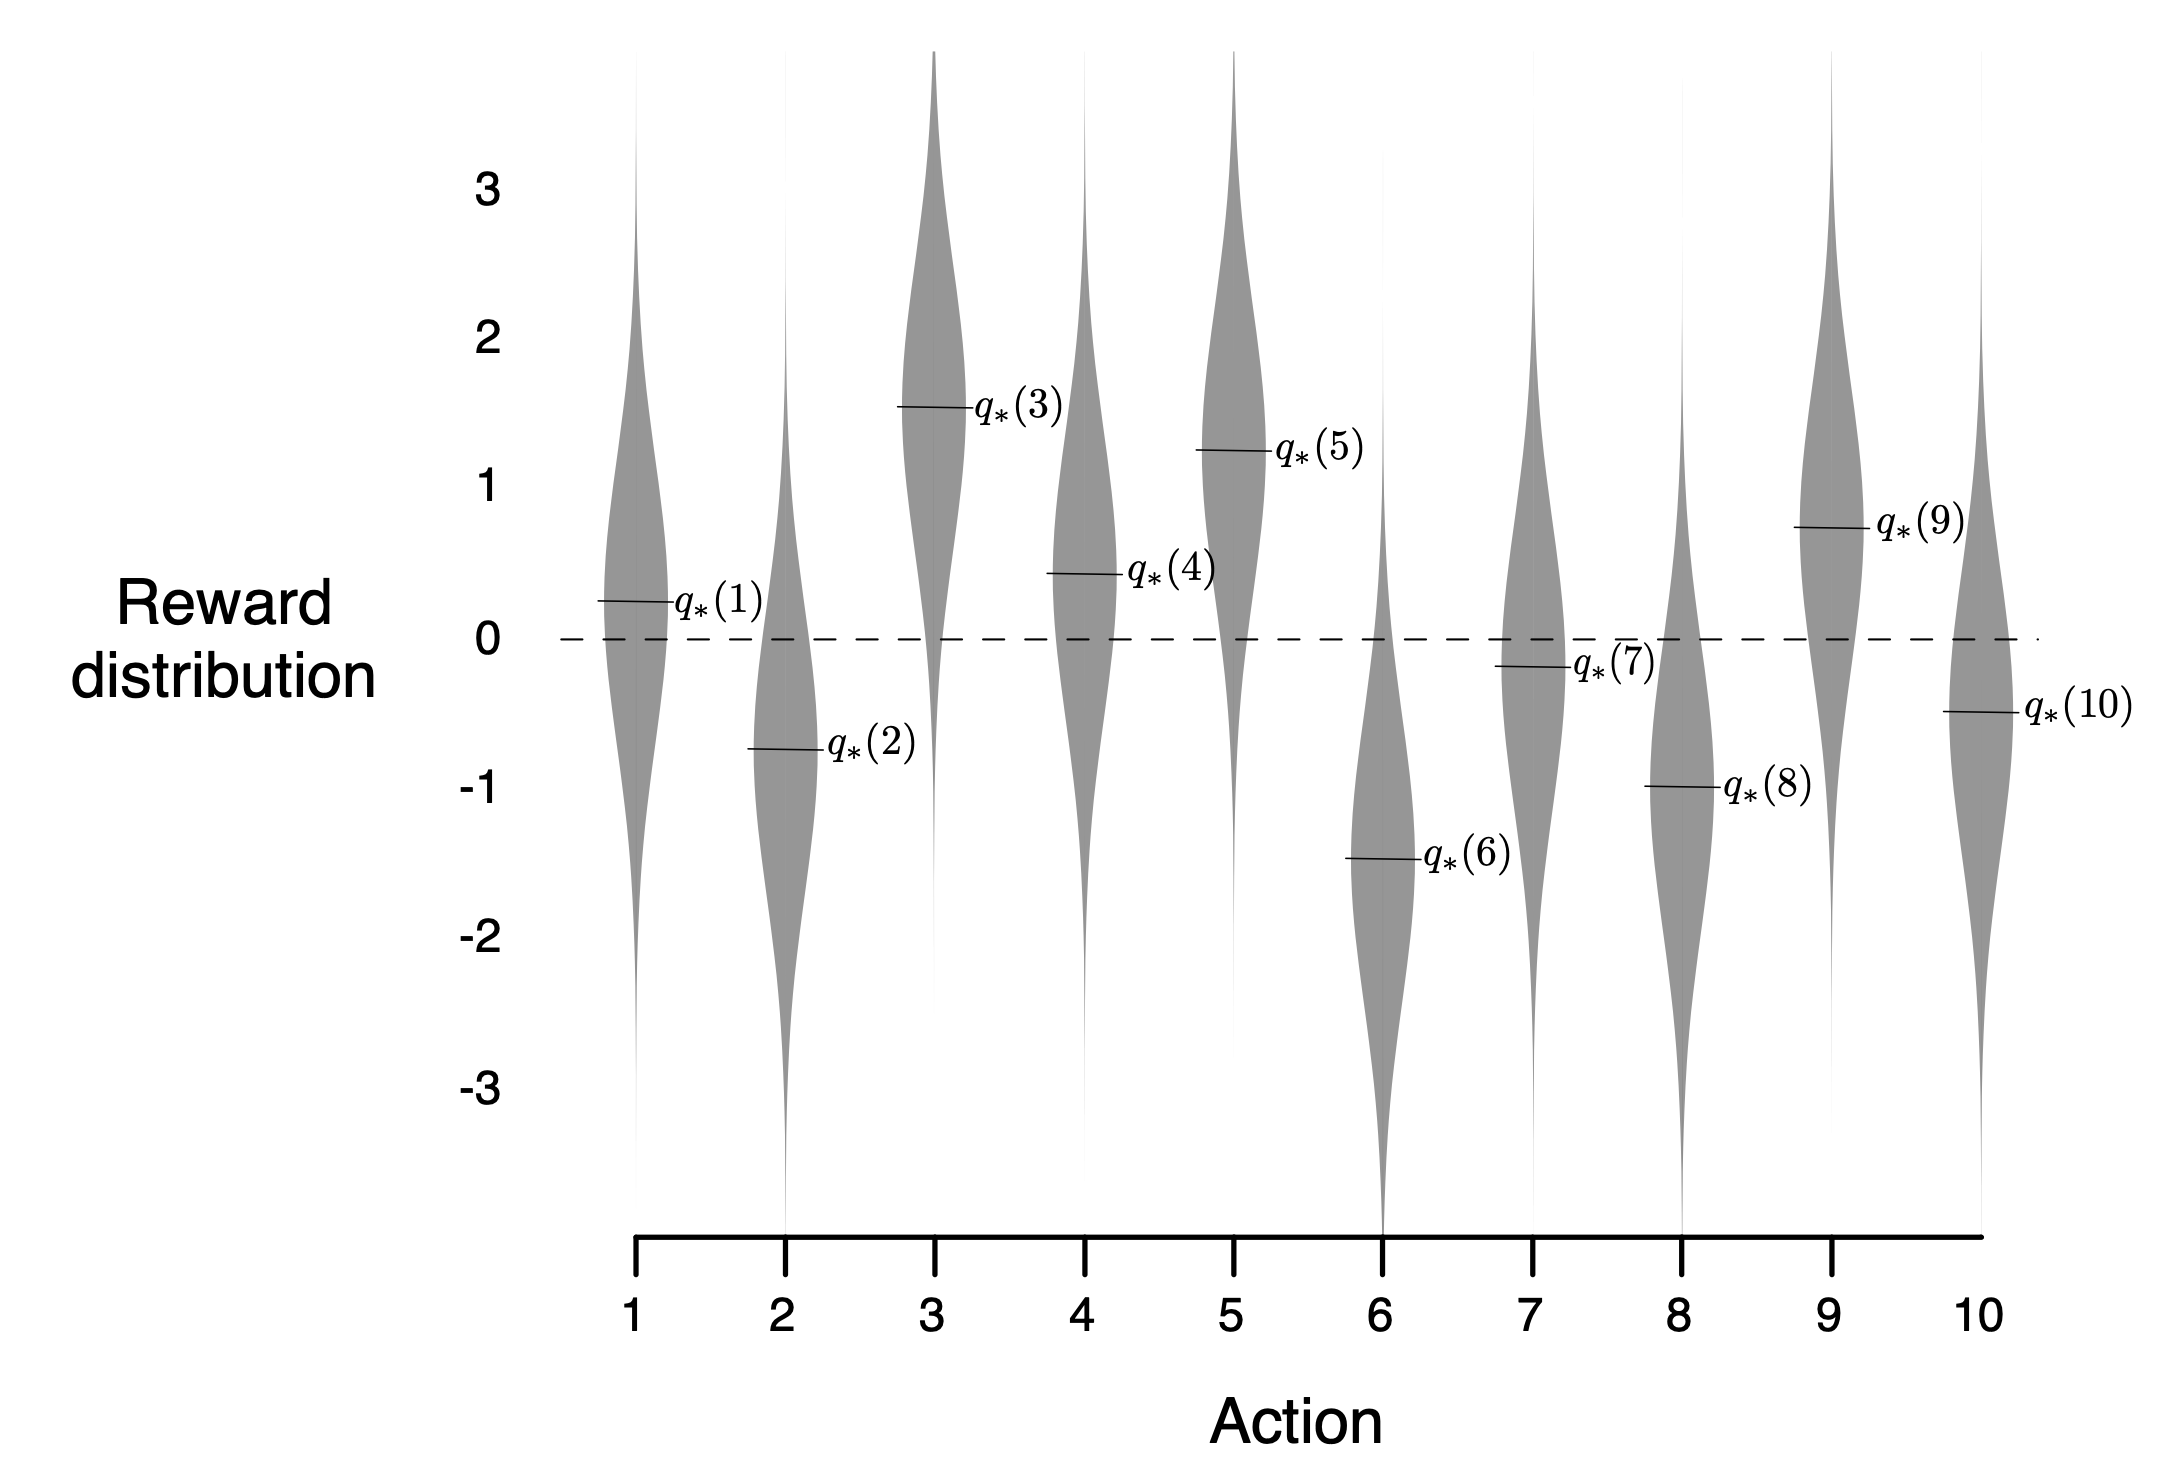
\includegraphics[width=0.9\textwidth]{fig/sutton_fig_2_1.png}
\caption{The $10$-armed bandit environment (Sutton and Barto, 2017, Fig. 2.1)}
\end{figure}

\end{frame}


\begin{frame}{Bandit example}

\begin{figure}[h]
\centering
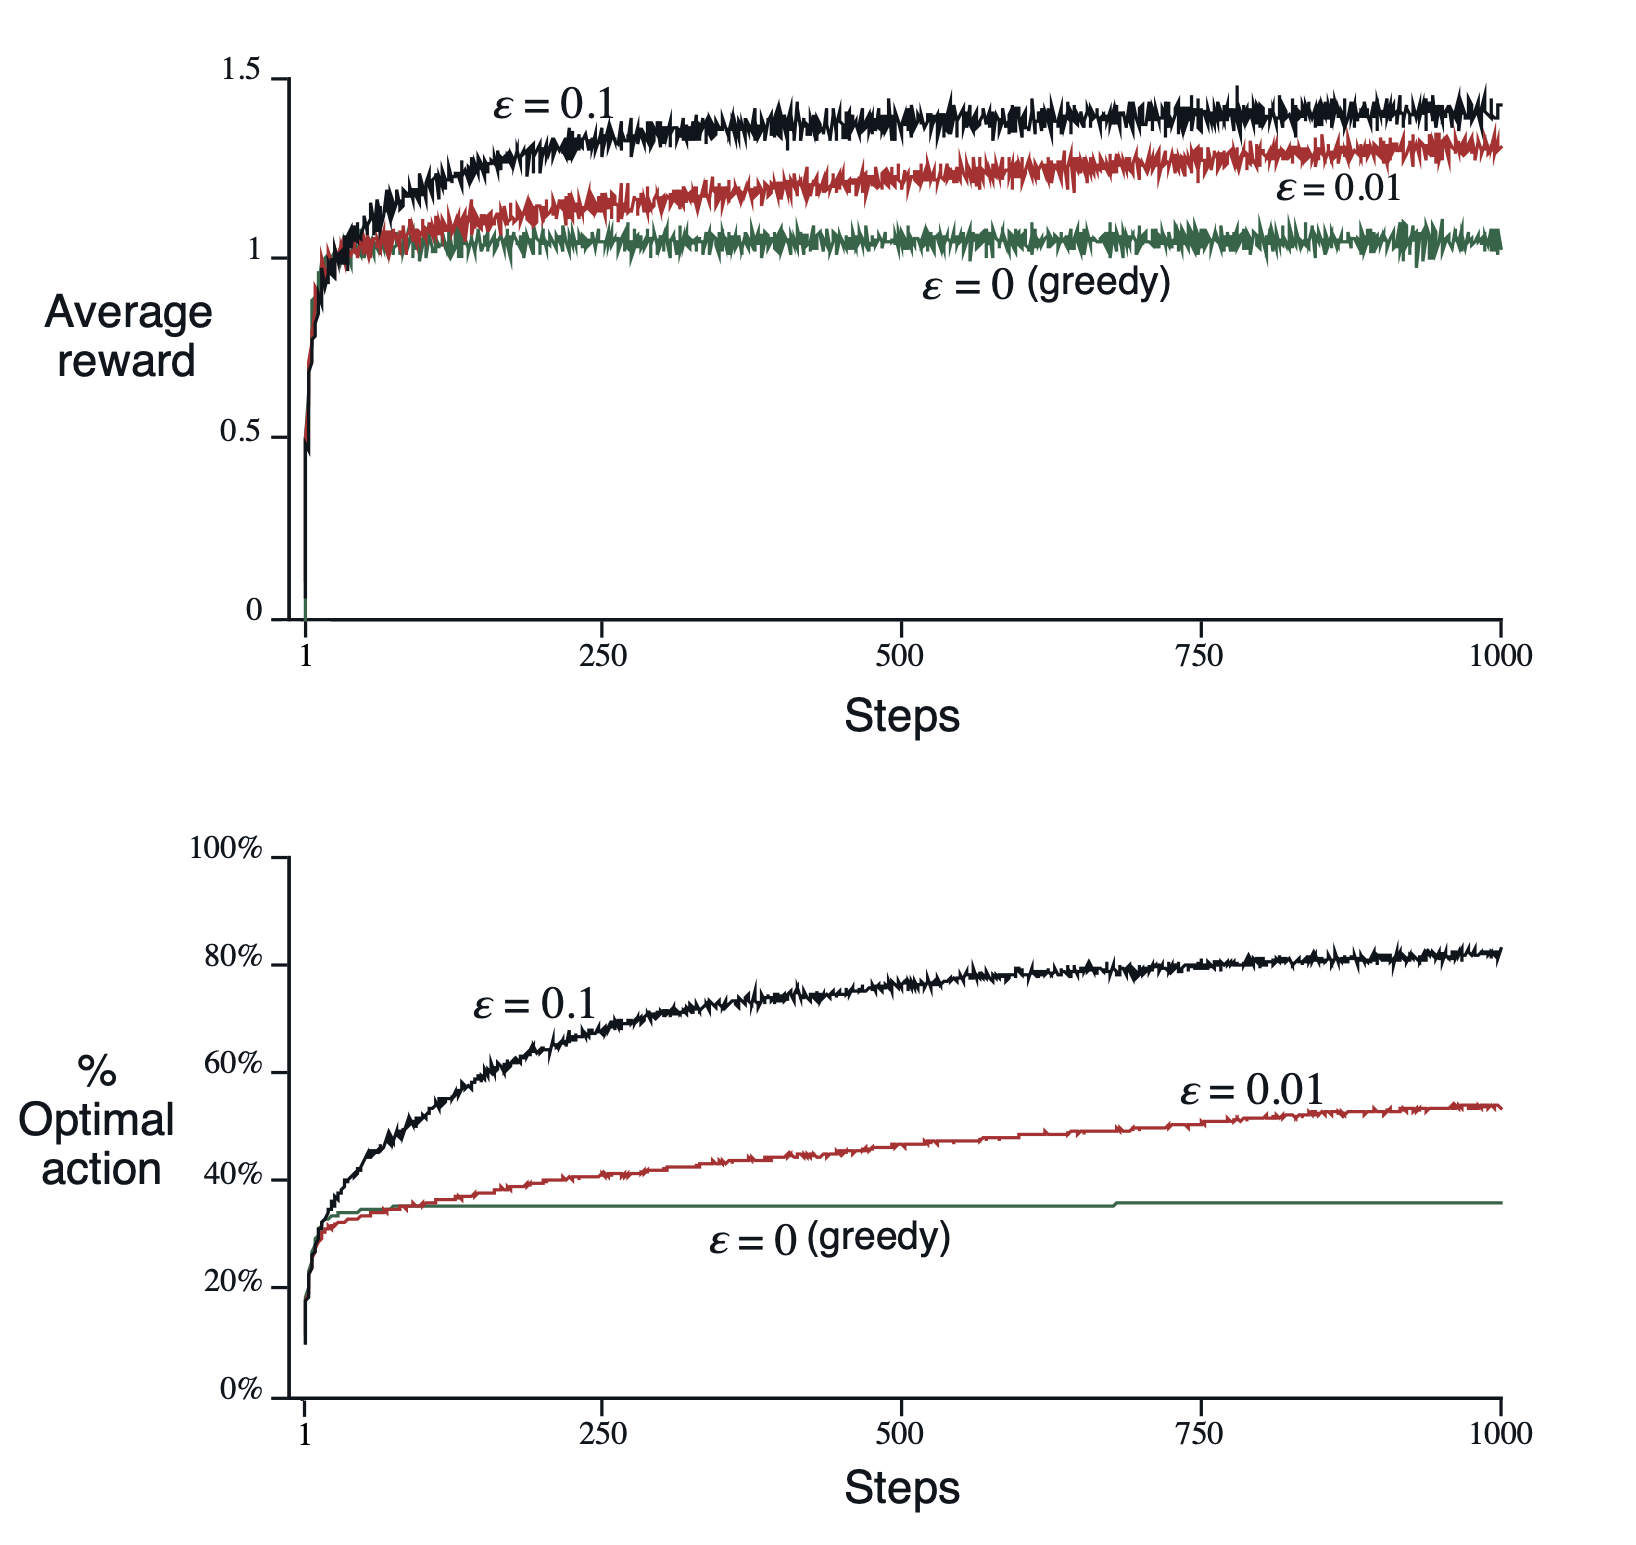
\includegraphics[width=0.7\textwidth]{fig/sutton_fig_2_2.png}
\caption{The $\epsilon$-greedy algorithm result in the 10-armed bandit (Sutton and Barto, 2017, Fig. 2.2)}
\end{figure}

\end{frame}


\begin{frame}{Bandit example: Optimistic initialization}

\begin{figure}[h]
\centering
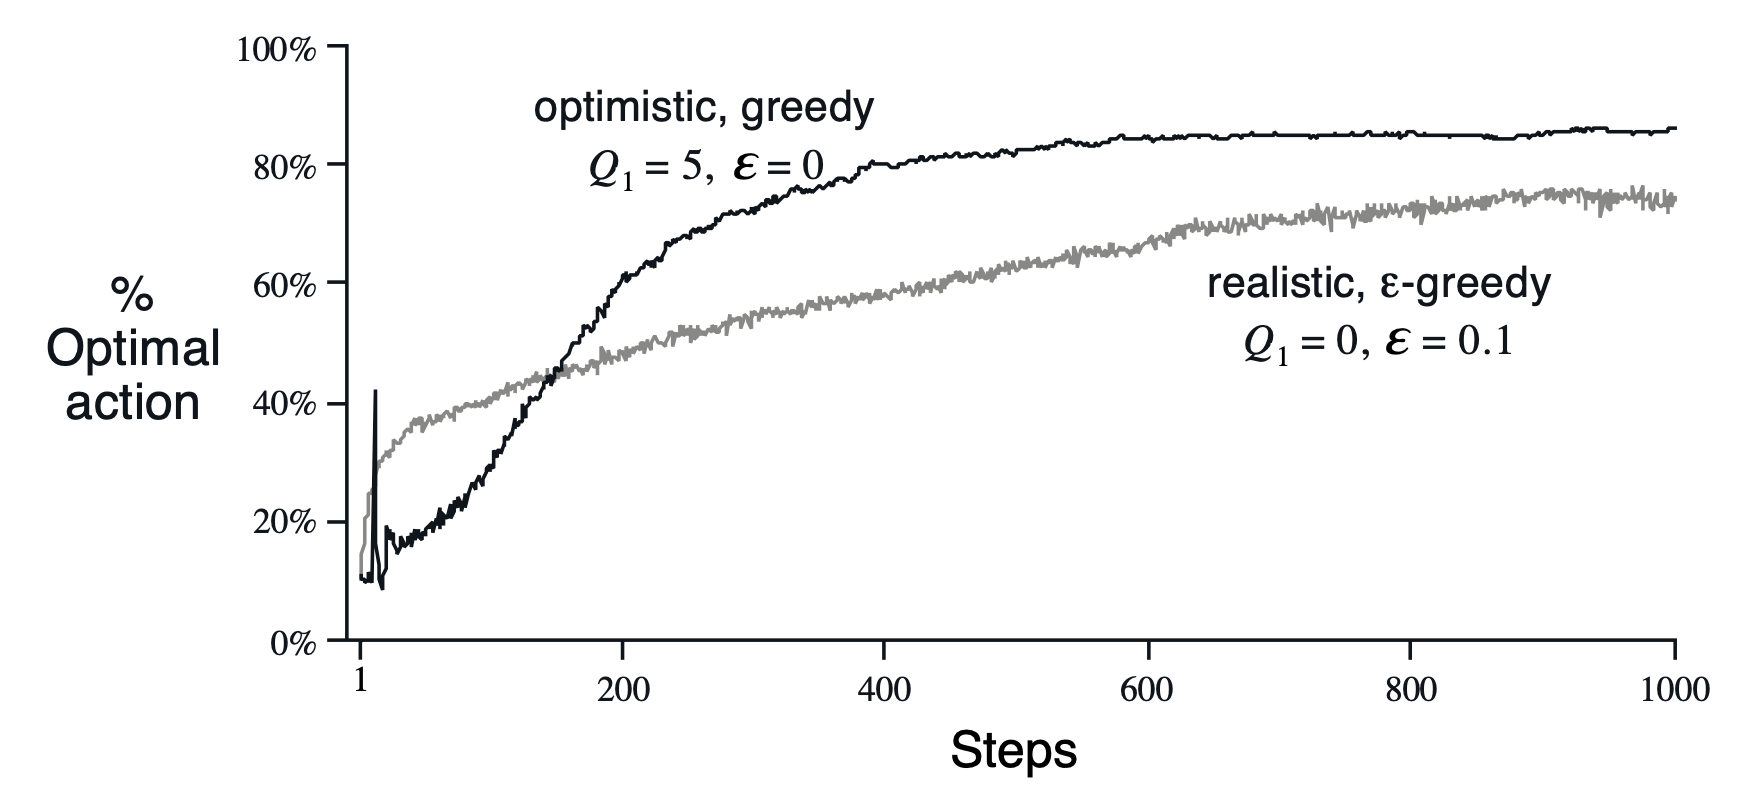
\includegraphics[width=0.9\textwidth]{fig/sutton_fig_2_3.png}
\caption{The $\epsilon$-greedy algorithm and optimistic initialization (Sutton and Barto, 2017, Fig. 2.3)}
\end{figure}

\end{frame}



\begin{frame}{Efficient computation and non-stationarity}

\begin{itemize}
\item Compute $Q_t(a)$ on the fly:
\[
Q_T(a) = Q_{T-1} + {\color{uured} \frac{1}{N_t(a)}} (R_{t,A_t=a} - Q_{T-1}(a))
\]
\pause
\item Handling non-stationarity:
\[
Q_T(a) = Q_{T-1} + {\color{uured} \alpha(t)} (R_{t, A_t=a} - Q_{T-1}(a))
\]
\end{itemize}

\end{frame}

\begin{frame}{Efficient computation and non-stationarity}

\[
Q_T(a) = Q_{T-1} + {\color{uured} \alpha(t)} (R_{t, A_t=a} - Q_{T-1}(a))
\]
\begin{itemize}
\item Examples:
\begin{itemize}
\item $\alpha(t) = 1$: $Q_T(a) = R_{t,A_t=a}$\pause
\item $\alpha(t) = 0$: $Q_T(a) = Q_{1}(a)$\pause
\item $\alpha(t) = \frac{1}{N_t(a)}$: Average reward\pause
\end{itemize}
\item $Q_T(a) \rightarrow q^\star(a)$, if:\pause
\begin{enumerate}
\item $\sum^\infty_t \alpha_t = \infty$
\item $\sum^\infty_t \alpha^2_t < \infty$
\end{enumerate}
\item Where have we seen these criterias before?
\end{itemize}

\end{frame}

\begin{frame}{The $\epsilon$-greedy algorithm}

\begin{figure}[h]
\centering
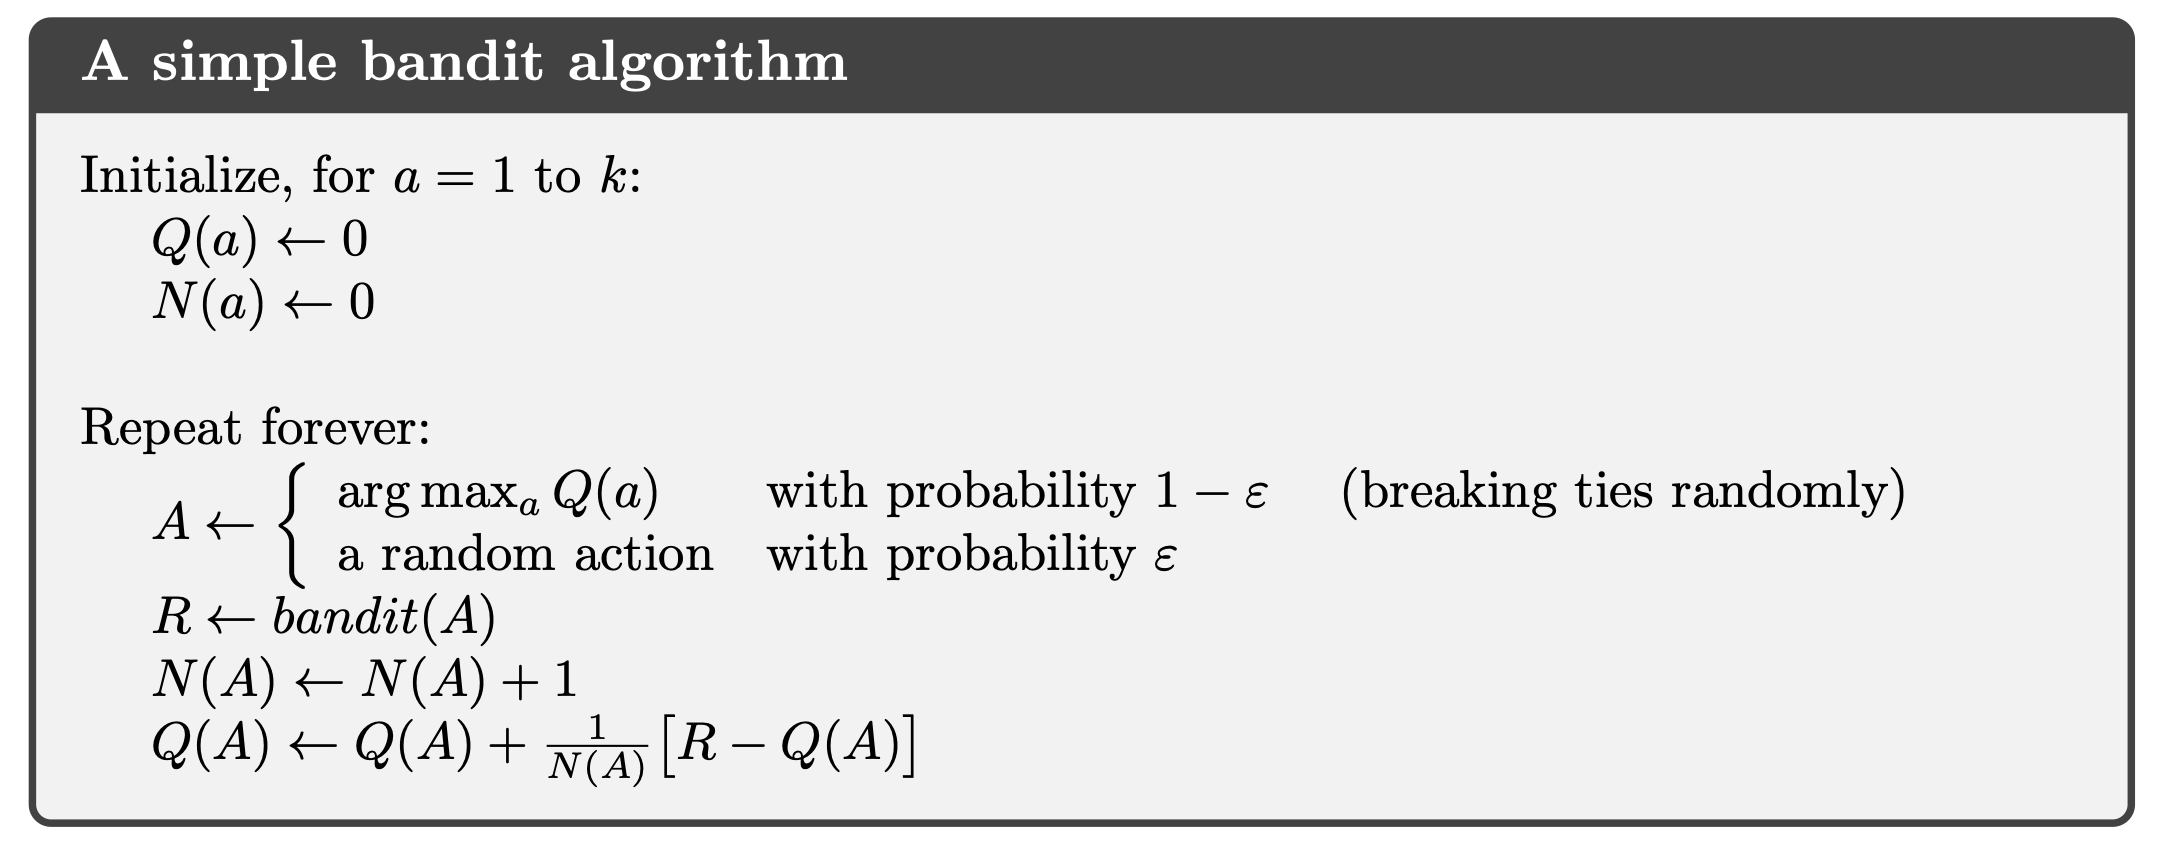
\includegraphics[width=1\textwidth]{fig/sutton_bandit.png}
\caption{The $\epsilon$-greedy algorithm}
\end{figure}

\end{frame}



\begin{frame}{The Upper-Confidence-Bound method}

\begin{itemize}
\item Explore based on our uncertainty of $Q_t(a)$\pause
\item The Upper-Confidence-Bound (UCB) method
\[
A_t = \arg \max_a \left( Q_{t} + c \sqrt{\frac{{\color{uured} \log t}}{N_t(a)}}  \right)
\]
An analogy:
\[
A_t = \arg \max_a \left( Q_{t} + c \sqrt{\frac{{\color{uured}\hat{\sigma}^2(a)}}{N_t(a)}} \right)
\]
\end{itemize}

\end{frame}


\begin{frame}{The UCB algorithm}

\begin{figure}[h]
\centering
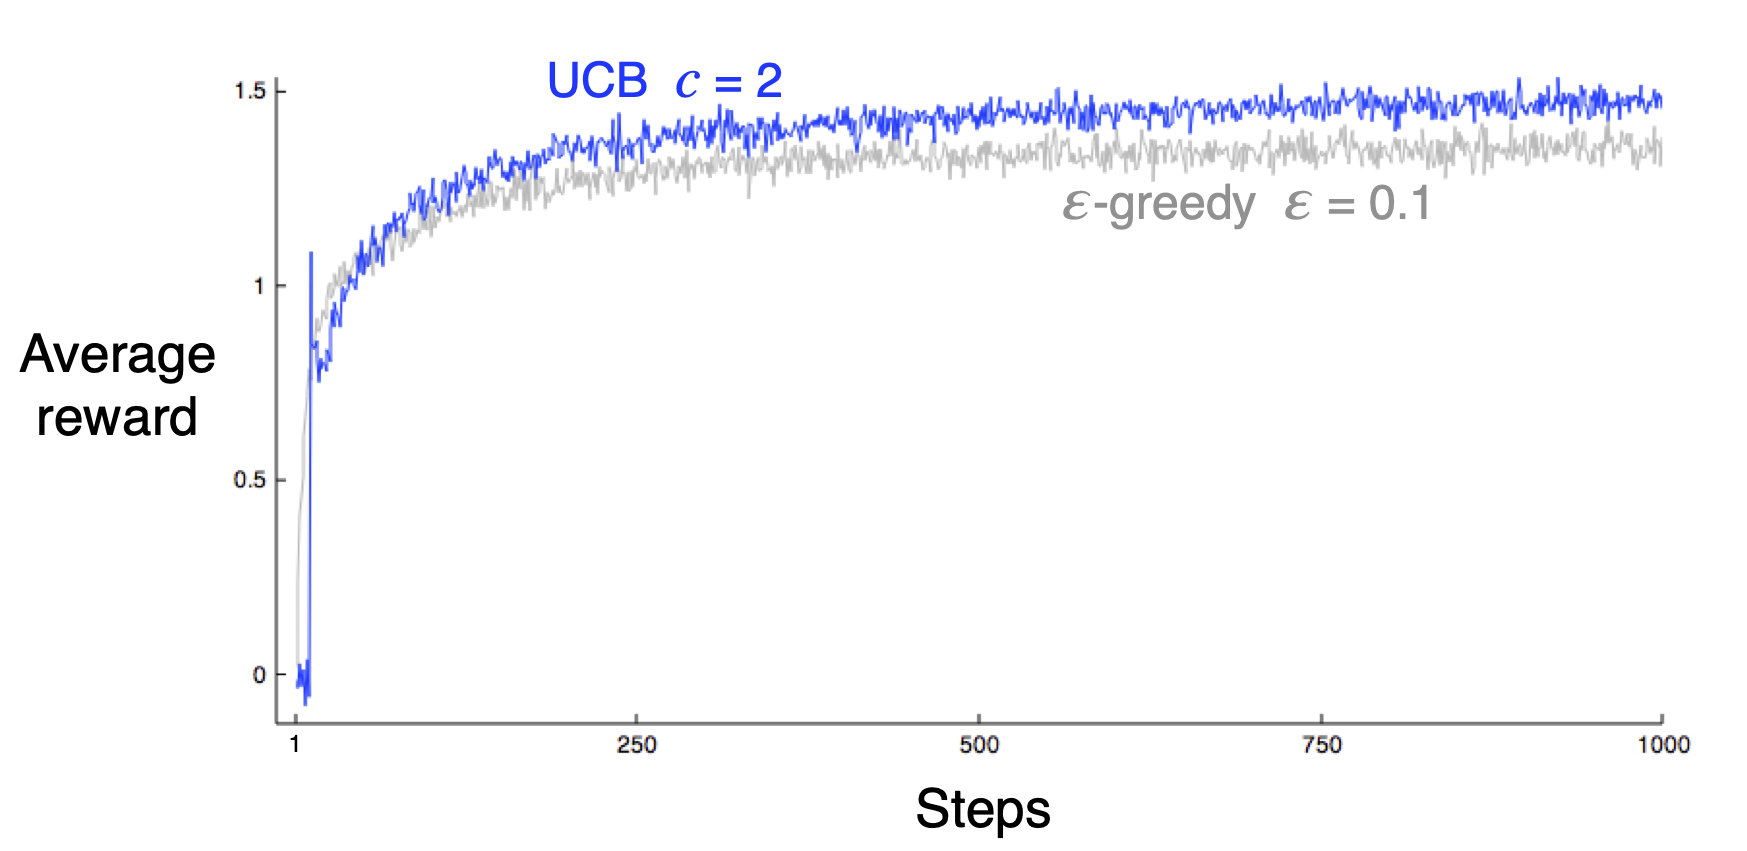
\includegraphics[width=0.9\textwidth]{fig/sutton_fig_2_4.png}
\caption{The UCB algorithm}
\end{figure}

\end{frame}

% TODO: Add gradient bandits


\begin{frame}{The Bayesian Bandit: Thompson sampling}

\begin{itemize}
\item A Bayesian Bandit
\begin{enumerate}
\item Setup a likelihood for $R$, $p(R|a,\theta)$
\item Setup a prior for $\theta$, $p(\theta)$
\item Compute posterior for $\theta$, $p(\theta|R, a)$
\item Choose action $A_t$ proportional to
\[
\int I[\E(R|\theta,a^\star) = \arg \max_{a'} \E(R|\theta,a')] p(\theta|R,a) d\theta
\]
where $I$ is the indicator function.
\end{enumerate}
\item Repeat step 3-4 \pause
\item Monte Carlo approximation of step 4:
\begin{enumerate}
\item Draw one sample from the posterior $\tilde{\theta}$
\[
\tilde{\theta} \sim p(\theta|R, a)
\]
\item Conditional on $\tilde{\theta}$, choose action $A_t$
\[
A_t = \arg \max_{a'} \E(R|\tilde{\theta},a')]
\]
\end{enumerate}

\end{itemize}

\end{frame}




\section{Markov Decision Processes}
\frame{\sectionpage}


\begin{frame}{The Markov Decision process}

\begin{itemize}
\item Bandits does not have a \emph{state}.\pause
\item An action might {\color{uured}change} the environment.
\item An action might be different in different {\color{uured}states}\pause
\item {\color{uured}Example}: In chess, we want to make a move based on the current position of all pieces\pause
\item To capture this we use a {\color{uured}Markov Decision process}
\item One of the most important concepts in Reinforcement Learning
\end{itemize}

\end{frame}





\begin{frame}{The Markov Decision process}

\begin{figure}[h]
\centering
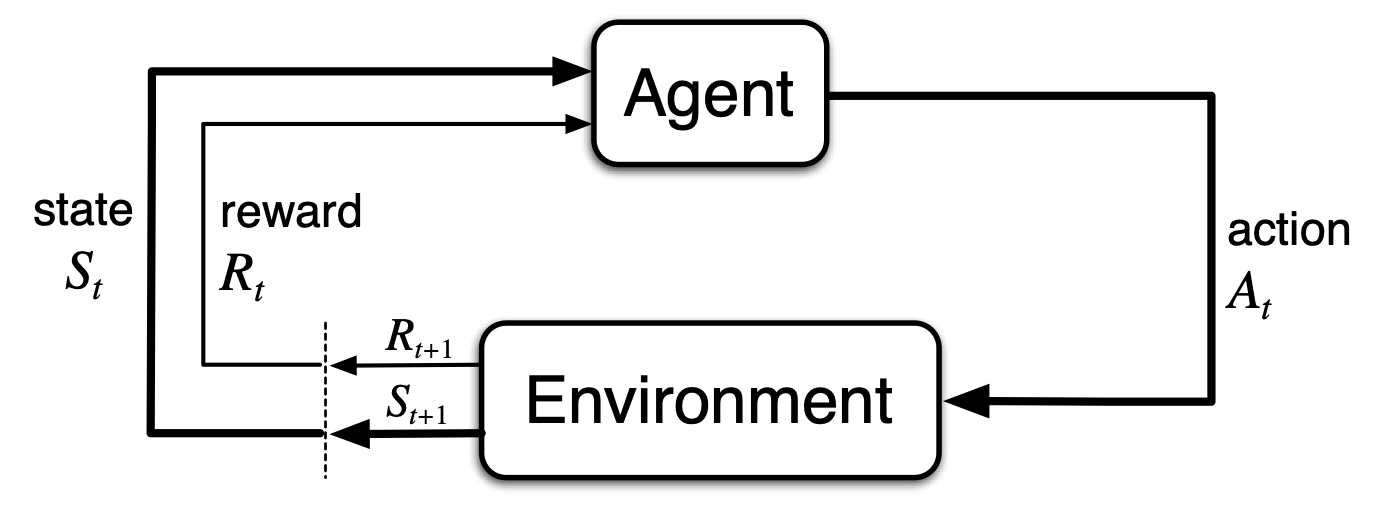
\includegraphics[width=0.9\textwidth]{fig/sutton_fig_3_1.png}
\caption{The (finite) Markov Decision Process (Sutton and Barto, 2017, Fig 3.1)}
\end{figure}

\begin{itemize}
\item States $S_t \in \mathcal{S}$: Basis for action
\item Actions $A_t \in \mathcal{A}$
\item Rewards $R_t \in \mathbb{R}$
\end{itemize}

\end{frame}


\begin{frame}{The Markov Decision process}

\begin{itemize}
\item Boundry between Agent and Environment:
\begin{itemize}
\item The {\color{uured}total control} of the action\pause
\item Reward is {\color{uured}external} to agent: Pain and pleasure
\item The agent {\color{uured} should not be able to change the reward function}
\end{itemize}
\pause
\item The policy ($\pi(A_t|S_t=s)$):
\begin{itemize}
\item We make an action given the current state $S_t$
\end{itemize}
\item {\color{uured}The goal}: (Again) maximize return $G_t = R_{t+1} + ... + R_{T}$
\end{itemize}

\end{frame}



\begin{frame}{Return and discount}

\begin{itemize}
\item Two type of interactions
\begin{itemize}
\item {\color{uured}Episodic}: $T <\infty$, has terminal state
\item {\color{uured}Continuing}: $T =\infty$
\end{itemize}
%\pause
\item Discounting:
\[
G_t = R_{t+1} + \gamma R_{t+3} + \gamma^2 R_{t+3} + ... = \sum^\infty_{k=0} \gamma^k R_{t+k+1}
\]
\pause
\item Discount rate $\gamma$:
\begin{itemize}
\item $0 \leq \gamma \leq 1$\pause
\item $\gamma = 1$: {\color{uured}No discount}
\item $\gamma = 0$: {\color{uured}Full discount}: Only next reward counts
\item $\gamma < 1$ and $R_t$ is bounded: $G_t<\infty$
\end{itemize}
\pause
\item For episodic problem we assume $R_{T+i} = 0$ for all $i \in \mathbb{N}^+$
\end{itemize}

\end{frame}

\begin{frame}{The Markov Decision Process}

\begin{itemize}
\item The Markov Decision process (MDP):
\[
P(S_{t+1} = s', R_{t+1} = r| S_t = s, A_t = a)\,\,(1)
\]
\item Eq. (1) {\color{uured}fully specify} a MDP
\pause
\item Markov property:
\begin{align*}
       P(S_{t+1} = s', R_{t+1} = r| S_1 = s, A_1 = a , ..., S_t = s, A_t = a) &  = \\
       P(S_{t+1} = s', R_{t+1} = r| S_t = s, A_t = a) &
\end{align*}
\item The MDP is a good {\color{uured} approximation or model}:\\
      All models are wrong, but some are useful.
\end{itemize}

\end{frame}



\begin{frame}{The Markov Decision Process Marginals}

\begin{itemize}
\item The Markov Decision process (MDP):
\[
P(S_{t+1} = s', R_{t+1} = r| S_t = s, A_t = a)\,\,(1)
\]
\item From Eq. (1) we can get marginals of interest:
\begin{itemize}
\item State-action rewards:
\[
r(s,a) = \mathbb{E}(R_{t+1}|S_t=s, A_t=a)
\]\pause
\item State-transition probability:
\[
p(s'|s,a) = P(S_{t+1}=s'|S_t=s, A_t=a)
\]
\end{itemize}
\end{itemize}

\end{frame}



\begin{frame}{The Value function}

\begin{itemize}
\item The value function $v_{\pi}(s)$: \\the long-term value of $s$ given a policy $\pi(a|s)$, i.e.
\[
v_{\pi}(s) = \mathbb{E}_\pi(G_t|S_t = s) = \mathbb{E}_\pi\left(\sum^\infty_{k=0} \gamma^k R_{t+k+1} | S_t=s \right)
\]
\pause
\item Informally: How "good" is a state for the agent with the policy $\pi$.

\end{itemize}

\end{frame}


\begin{frame}{The Value function}

\begin{itemize}
\item Estimating $v_{\pi}(s)$ is one of the most important problem in RL\pause
\item Value functions are {\color{uured}recursive}:
\begin{align*}
       v_{\pi}(s) & = \mathbb{E}_\pi(G_t|S_t = s)      \\
                  & = \sum_a \pi(a|s) \sum_{s',r} p(s', r|s,a) (r + \gamma v_{\pi}(s'))
\end{align*}
\item This is the {\color{uured}Bellman equation} for $v_\pi(s)$: \\The relationship between the values of the state and its successor states.\pause
\item Bellman equation is the basis for computing $v_\pi(s)$ (not part of this course)

\end{itemize}

\end{frame}



\begin{frame}{The value function}

\begin{figure}[h]
\centering
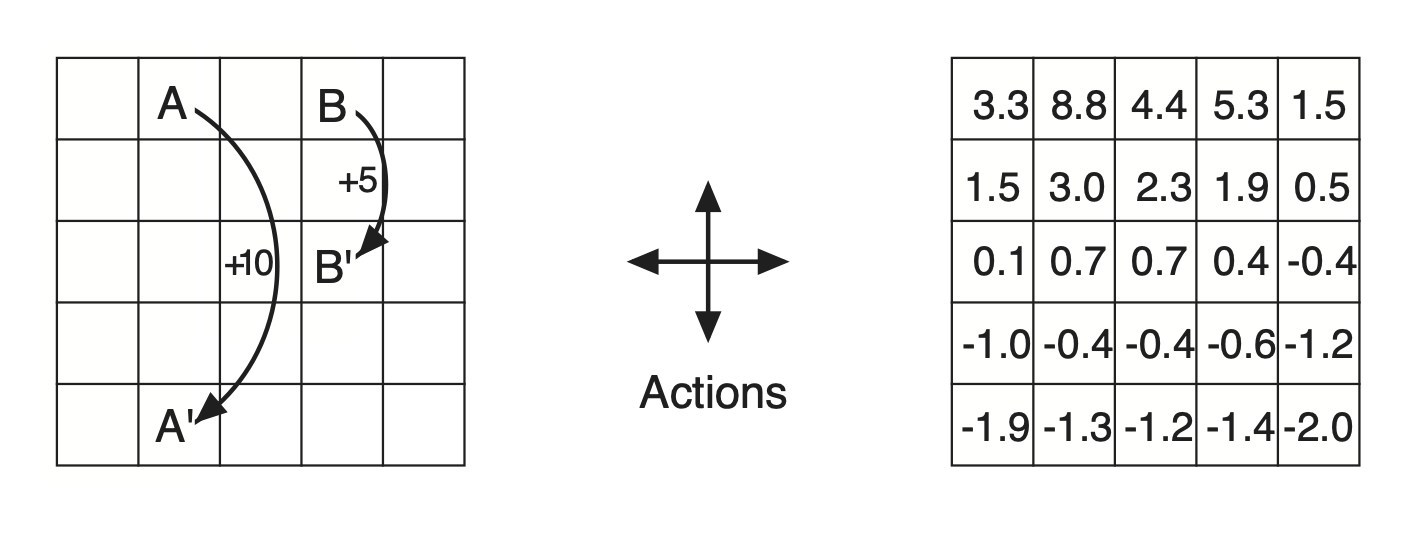
\includegraphics[width=0.9\textwidth]{fig/sutton_fig_3_5.png}
\caption{The gridworld equiprobable policy value function}
\end{figure}

\end{frame}

\begin{frame}{The Optimal Policy}

\begin{itemize}
\item A policy $\pi$ is {\color{uured}better} than $\pi'$ if $v_\pi(s) \geq v_{\pi'}(s)$ for all $s \in \mathcal{S}$.\pause
\item A policy that is better or equal to all other policies is the {\color{uured}optimal policy} $\pi_\star$.\pause
\item The optimal value function: $v_{\pi_\star}(s) = v_\star(s)$\pause
\item The optimal policy $\pi_\star$ is greedy wrt $v_{\pi_\star}(s)$: \\The best long term strategy
\end{itemize}

\end{frame}

\begin{frame}{The Optimal Policy}

\begin{itemize}
\item Computing optimal value function might be {\color{uured}impossible}:\\ we need to estimate/re-estimate/approximate it
\item {\color{uured}Example}: Chess, we cannot compute the optimal long-term moves, we need to approximate/estimate (based on computational budget)\pause
\item We might also estimate $v_\star(s)$ better for commonly encountered states
\end{itemize}

\end{frame}

\begin{frame}{The value function}

\begin{figure}[h]
\centering
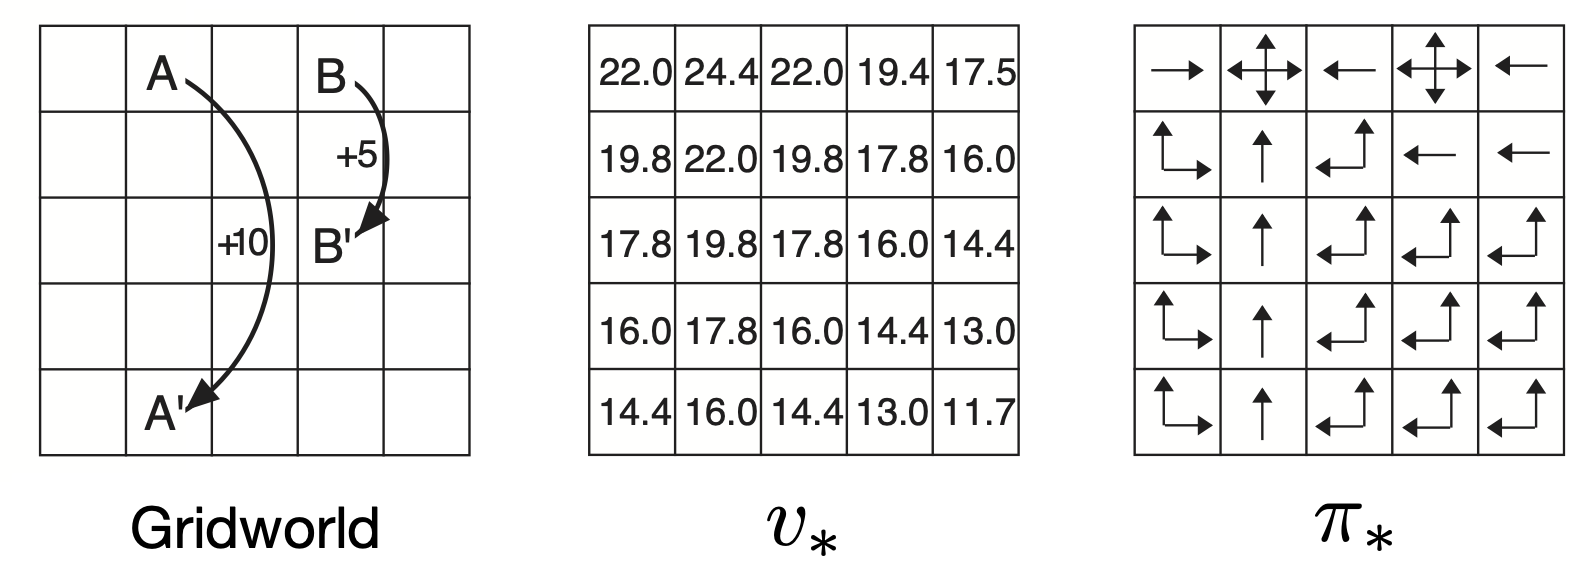
\includegraphics[width=0.9\textwidth]{fig/sutton_fig_3_8.png}
\caption{The gridworld optimal value function and policy}
\end{figure}

\end{frame}


\end{document}
